%%%%%%%%%%%%%%%%%%%%%%%%%%%%%%%%%%%%%%%%%%%%%%%%%%%%%%%%%%%%%%%%%%%%%%%%%%%%%%%%
%% Plantilla de memoria en LaTeX para la ETSIT - Universidad Rey Juan Carlos
%%
%% Por Gregorio Robles <grex arroba gsyc.urjc.es>
%%     Grupo de Sistemas y Comunicaciones
%%     Escuela Técnica Superior de Ingenieros de Telecomunicación
%%     Universidad Rey Juan Carlos
%% (muchas ideas tomadas de Internet, colegas del GSyC, antiguos alumnos...
%%  etc. Muchas gracias a todos)
%%
%% La última versión de esta plantilla está siempre disponible en:
%%     https://github.com/gregoriorobles/plantilla-memoria
%%
%% Para obtener PDF, ejecuta en la shell:
%%   make
%% (las imágenes deben ir en PNG o JPG)

%%%%%%%%%%%%%%%%%%%%%%%%%%%%%%%%%%%%%%%%%%%%%%%%%%%%%%%%%%%%%%%%%%%%%%%%%%%%%%%%

\documentclass[a4paper, 12pt]{book}
%\usepackage[T1]{fontenc}

\usepackage[a4paper, left=2.5cm, right=2.5cm, top=3cm, bottom=3cm]{geometry}
\usepackage{times}
\usepackage[utf8]{inputenc}
\usepackage[spanish]{babel} % Comenta esta línea si tu memoria es en inglés
\usepackage{url}
%\usepackage[dvipdfm]{graphicx}
\usepackage{graphicx}
\usepackage{float}  %% H para posicionar figuras
\usepackage[nottoc, notlot, notlof, notindex]{tocbibind} %% Opciones de índice
\usepackage{latexsym}  %% Logo LaTeX
\usepackage{dirtree}
\usepackage{tikz}
\usepackage{listings}


\usetikzlibrary{shapes,arrows}
\tikzstyle{decision} = [diamond, draw, 
    text width=4.5em, text badly centered, node distance=3cm, inner sep=0pt]
\tikzstyle{block} = [rectangle, draw,  
    text width=5em, text centered, rounded corners, minimum height=4em]
\tikzstyle{line} = [draw, -latex']


\title{Memoria del Proyecto}
\author{Nombre del autor}

\renewcommand{\baselinestretch}{1.5}  %% Interlineado

\begin{document}

\renewcommand{\refname}{Bibliografía}  %% Renombrando
\renewcommand{\appendixname}{Apéndice}

\lstset{frame=L,breaklines=true,keepspaces=true,basicstyle=\footnotesize, language=Python,showstringspaces=false} 

%%%%%%%%%%%%%%%%%%%%%%%%%%%%%%%%%%%%%%%%%%%%%%%%%%%%%%%%%%%%%%%%%%%%%%%%%%%%%%%%
% PORTADA

\begin{titlepage}
\begin{center}
\begin{tabular}[c]{c c}
%\includegraphics[bb=0 0 194 352, scale=0.25]{logo} &
\includegraphics[scale=0.25]{img/logo_vect.png} &
\begin{tabular}[b]{l}
\Huge
\textsf{UNIVERSIDAD} \\
\Huge
\textsf{REY JUAN CARLOS} \\
\end{tabular}
\\
\end{tabular}

\vspace{3cm}

\Large
INGENIERÍA EN TELECOMUNICACIONES Y LICENCIATURA EN ADMINISTRACIÓN Y DIRECCIÓN DE EMPRESAS

\vspace{0.4cm}

\large
Curso Académico 2016/2017

\vspace{0.8cm}

Trabajo Fin de Carrera

\vspace{2.5cm}

\LARGE
MY APP ANALYZER: fomentando el desarrollo web entre los jóvenes

\vspace{4cm}

\large
Autor : Alexandra Ortega Martín \\
Tutor : Dr. Gregorio Robles
\end{center}
\end{titlepage}

\newpage
\mbox{}
\thispagestyle{empty} % para que no se numere esta pagina


%%%%%%%%%%%%%%%%%%%%%%%%%%%%%%%%%%%%%%%%%%%%%%%%%%%%%%%%%%%%%%%%%%%%%%%%%%%%%%%%
%%%% Para firmar
\clearpage
\pagenumbering{gobble}
\chapter*{}

\vspace{-4cm}
\begin{center}
\LARGE
\textbf{Proyecto Fin de Carrera}

\vspace{1cm}
\large
My App Analyzer: fomentando el desarrollo web entre los jóvenes

\vspace{1cm}
\large
\textbf{Autor :} Alexandra Ortega Martín \\
\textbf{Tutor :} Dr. Gregorio Robles Martínez

\end{center}

\vspace{1cm}
La defensa del presente Proyecto Fin de Carrera se realizó el día \qquad$\;\,$ de \qquad\qquad\qquad\qquad \newline de 2017, siendo calificada por el siguiente tribunal:


\vspace{0.5cm}
\textbf{Presidente:}

\vspace{1.2cm}
\textbf{Secretario:}

\vspace{1.2cm}
\textbf{Vocal:}


\vspace{1.2cm}
y habiendo obtenido la siguiente calificación:

\vspace{1cm}
\textbf{Calificación:}


\vspace{1cm}
\begin{flushright}
Fuenlabrada, a \qquad$\;\,$ de \qquad\qquad\qquad\qquad de 2017
\end{flushright}

%%%%%%%%%%%%%%%%%%%%%%%%%%%%%%%%%%%%%%%%%%%%%%%%%%%%%%%%%%%%%%%%%%%%%%%%%%%%%%%%
%%%% Dedicatoria

\chapter*{}
\pagenumbering{Roman} % para comenzar la numeracion de paginas en numeros romanos
\begin{flushright}
\textit{Dedicado a \\
mi familia / mi abuelo / mi abuela}
\end{flushright}

%%%%%%%%%%%%%%%%%%%%%%%%%%%%%%%%%%%%%%%%%%%%%%%%%%%%%%%%%%%%%%%%%%%%%%%%%%%%%%%%
%%%% Agradecimientos

\chapter*{Agradecimientos}
%\addcontentsline{toc}{chapter}{Agradecimientos} % si queremos que aparezca en el índice
\markboth{AGRADECIMIENTOS}{AGRADECIMIENTOS} % encabezado 

Aquí vienen los agradecimientos\ldots Aunque está bien acordarse de la pareja,
no hay que olvidarse de dar las gracias a tu madre, que aunque a veces no lo 
parezca disfrutará tanto de tus logros como tú\ldots Además, la pareja quizás
no sea para siempre, pero tu madre sí.

%%%%%%%%%%%%%%%%%%%%%%%%%%%%%%%%%%%%%%%%%%%%%%%%%%%%%%%%%%%%%%%%%%%%%%%%%%%%%%%%
%%%% Resumen

\chapter*{Resumen}
%\addcontentsline{toc}{chapter}{Resumen} % si queremos que aparezca en el índice
\markboth{RESUMEN}{RESUMEN} % encabezado

Aquí viene un resumen del proyecto. Ha de constar de tres o cuatro párrafos,
donde se presente de manera clara y concisa de qué va el proyecto. Han
de quedar respondidas las siguientes preguntas:

\begin{itemize}
  \item ¿De qué va este proyecto? ¿Cuál es su objetivo principal?
  \item ¿Cómo se ha realizado? ¿Qué tecnologías están involucradas?
  \item ¿En qué contexto se ha realizado el proyecto? ¿Es un proyecto
dentro de un marco general?
\end{itemize}

Lo mejor es escribir el resumen al final.

%%%%%%%%%%%%%%%%%%%%%%%%%%%%%%%%%%%%%%%%%%%%%%%%%%%%%%%%%%%%%%%%%%%%%%%%%%%%%%%%
%%%% Resumen en inglés

\chapter*{Summary}
%\addcontentsline{toc}{chapter}{Summary} % si queremos que aparezca en el índice
\markboth{SUMMARY}{SUMMARY} % encabezado

Here comes a translation of the ``Resumen'' into English. Please, double check
it for correct grammar and spelling. As it is the translation of the ``Resumen'',
which is supposed to be written at the end, this as well should be filled out
just before submitting.


%%%%%%%%%%%%%%%%%%%%%%%%%%%%%%%%%%%%%%%%%%%%%%%%%%%%%%%%%%%%%%%%%%%%%%%%%%%%%%%%
%%%%%%%%%%%%%%%%%%%%%%%%%%%%%%%%%%%%%%%%%%%%%%%%%%%%%%%%%%%%%%%%%%%%%%%%%%%%%%%%
% ÍNDICES %
%%%%%%%%%%%%%%%%%%%%%%%%%%%%%%%%%%%%%%%%%%%%%%%%%%%%%%%%%%%%%%%%%%%%%%%%%%%%%%%%

% Las buenas noticias es que los índices se generan automáticamente.
% Lo único que tienes que hacer es elegir cuáles quieren que se generen,
% y comentar/descomentar esa instrucción de LaTeX.

%%%% Índice de contenidos
\tableofcontents 
%%%% Índice de figuras
\cleardoublepage
%\addcontentsline{toc}{chapter}{Lista de figuras} % para que aparezca en el indice de contenidos
\listoffigures % indice de figuras
%%%% Índice de tablas
%\cleardoublepage
%\addcontentsline{toc}{chapter}{Lista de tablas} % para que aparezca en el indice de contenidos
%\listoftables % indice de tablas


%%%%%%%%%%%%%%%%%%%%%%%%%%%%%%%%%%%%%%%%%%%%%%%%%%%%%%%%%%%%%%%%%%%%%%%%%%%%%%%%
%%%%%%%%%%%%%%%%%%%%%%%%%%%%%%%%%%%%%%%%%%%%%%%%%%%%%%%%%%%%%%%%%%%%%%%%%%%%%%%%
% INTRODUCCIÓN %
%%%%%%%%%%%%%%%%%%%%%%%%%%%%%%%%%%%%%%%%%%%%%%%%%%%%%%%%%%%%%%%%%%%%%%%%%%%%%%%%

\cleardoublepage
\chapter{Introducción}
\label{sec:intro} % etiqueta para poder referenciar luego en el texto con ~\ref{sec:intro}
\pagenumbering{arabic} % para empezar la numeración de página con números

En este capítulo se introduce el proyecto. Debería tener información general sobre 
el mismo, dando la información sobre el contexto en el que se ha desarrollado.

No te olvides de echarle un ojo a la página con los cinco errores de escritura más frecuentes\footnote{\url{http://www.tallerdeescritores.com/errores-de-escritura-frecuentes}}.

\section{}
\label{sec:}

\subsection{Estilo}
\label{subsec:estilo}

Sobre el uso de las comas\footnote{\url{http://narrativabreve.com/2015/02/opiniones-de-un-corrector-de-estilo-11-recetas-para-escribir-correctamente-la-coma.html}}

 \begin{figure}
    \centering
    \includegraphics[bb=0 0 800 600, width=12cm, keepaspectratio]{img/foro1}
    \caption{Página con enlaces a hilos}
    \label{figura:foro_hilos}
 \end{figure}

{\footnotesize
\begin{verbatim}
    From gaurav at gold-solutions.co.uk  Fri Jan 14 14:51:11 2005
    From: gaurav at gold-solutions.co.uk (gaurav_gold)
    Date: Fri Jan 14 19:25:51 2005
    Subject: [Mailman-Users] mailman issues
    Message-ID: <003c01c4fa40$1d99b4c0$94592252@gaurav7klgnyif>

    Dear Sir/Madam,
    How can people reply to the mailing list?  How do i turn off
    this feature? How can i also enable a feature where if someone
    replies the newsletter the email gets deleted?
    Thanks

    From msapiro at value.net  Fri Jan 14 19:48:51 2005
    From: msapiro at value.net (Mark Sapiro)
    Date: Fri Jan 14 19:49:04 2005
    Subject: [Mailman-Users] mailman issues
    In-Reply-To: <003c01c4fa40$1d99b4c0$94592252@gaurav7klgnyif>
    Message-ID: <PC173020050114104851057801b04d55@msapiro>

    gaurav_gold wrote:
    >How can people reply to the mailing list?  How do i turn off
    this feature? How can i also enable a feature where if someone
    replies the newsletter the email gets deleted?

    See the FAQ
    >Mailman FAQ: http://www.python.org/cgi-bin/faqw-mm.py
    article 3.11
\end{verbatim}
}

\section{Estructura de la memoria}
\label{sec:estructura}

En esta sección se debería introducir la esctura de la memoria. Así:

\begin{itemize}
  \item En el primer capítulo se hace una intro al proyecto.
  
  \item En el capítulo~\ref{chap:objetivos} se muestran los objetivos del proyecto.
  
  \item A continuación se presenta el estado del arte.
  
  \item \ldots
\end{itemize}



%%%%%%%%%%%%%%%%%%%%%%%%%%%%%%%%%%%%%%%%%%%%%%%%%%%%%%%%%%%%%%%%%%%%%%%%%%%%%%%%
%%%%%%%%%%%%%%%%%%%%%%%%%%%%%%%%%%%%%%%%%%%%%%%%%%%%%%%%%%%%%%%%%%%%%%%%%%%%%%%%
% OBJETIVOS %
%%%%%%%%%%%%%%%%%%%%%%%%%%%%%%%%%%%%%%%%%%%%%%%%%%%%%%%%%%%%%%%%%%%%%%%%%%%%%%%%

\cleardoublepage
\chapter{Objetivos}
\label{chap:objetivos}

\section{Objetivo general}
\label{sec:objetivo-general} El objetivo general de este proyecto es crear una plataforma donde los nuevos programadores puedan evaluar su código de forma que no sólo puedan conocer sus puntos fuertes y débiles sino que además puedan obtener nuevos retos para mejorar sus habilidades computacionales. 

Niños y jóvenes con interés por la programación conforman el público objetivo al que va destinada la aplicación. Por ello se han adaptado el diseño, funcionalidad y lenguaje para que resulten la experiencia de usuario sea lo más atractiva y lúdica posible. 

En el sistema de clasificación hemos huido de las puntuaciones númericas, convirtiéndolas en tres niveles representados por los colores del semáforo: alto (verde), medio (amarillo) y bajo (rojo). De esta manera convertimos la experiencia en un juego, enmarcándola en un contexto más positivo para el usuario y alejándonos de las puntuaciones númericas utilizadas de los exámenes. 

Toda la aplicación se relaciona con el usuario a través de un lenguaje coloquial, sencillo y en inglés. Se eligió este idioma porque es importante familizarizar a los niños con el mismo y reforzar sus conocimientos a través del juego.

\section{Objetivos específicos}
\label{sec:objetivos-especificos}
\begin{itemize}
  \item Analizar las posibilidades de personalización y bloques computacionales que ofrece App Inventor como herramienta para crear programas.

  \item Definir las habilidades y capacidades del usuario a analizar. De los múltiples enfoques considerados y de cara a una simplicación de la información final se optó por crear tres grandes bloques de análisis: componentes, programación y usabilidad.

  \item Crear una aplicación Django donde se recoja la lógica anterior y poder ofrecer al usuario la información de manera clara y resumida. El usuario podrá además tener un registro de los proyectos guardados con anterioridad para poder revisar su clasificación. 
  
  \item Unir las tecnologías Django, Bootstrap y Ajax para mejorar la capa de \textit{Front End} y hacer la experiencia de usuario mucho más dinámica.   
\end{itemize}


\section{Planificación temporal}
\label{sec:planificacion-temporal}
La planificación temporal del proyecto ha sido definida en función de los objetivos específicos marcados siguiendo un orden que permitiera avanzar en todos los aspectos de la aplicación:
\begin{itemize}
  \item \textbf{Fase I}: búsqueda de documentación sobre App Inventor y creación de una cuenta en su web \footnote{\url{http://appinventor.mit.edu/explore/}}donde poder analizar los bloques disponibles para el usuario, el contenido del archivo comprimido (\textit{.aia}) en que se guardan los programas y cómo se representa la información dentro del mismo. 

  \item \textbf{Fase II}: 
	\begin{itemize}
		\item Creación de una aplicación Django con una web simple donde subir el fichero con el proyecto, descomprimirlo y guardar su información en base de datos.
		\item Añadir la posibilidad de tener una cuenta de usuario en la aplicación donde se almacenen los diferentes proyectos subidos de cara a futuras consultas. 
	\end{itemize}
  \item \textbf{Fase III}: definición de los puntos a analizar en cada proyecto subido e implementar la lógica de evaluación y clasificación.
  
  
  \item \textbf{Fase IV}: incorporar a la web las tecnologías Bootstrap y Ajax para añadir dinamismo y mejorar su aspecto. 
\end{itemize}


%%%%%%%%%%%%%%%%%%%%%%%%%%%%%%%%%%%%%%%%%%%%%%%%%%%%%%%%%%%%%%%%%%%%%%%%%%%%%%%%
%%%%%%%%%%%%%%%%%%%%%%%%%%%%%%%%%%%%%%%%%%%%%%%%%%%%%%%%%%%%%%%%%%%%%%%%%%%%%%%%
% ESTADO DEL ARTE %
%%%%%%%%%%%%%%%%%%%%%%%%%%%%%%%%%%%%%%%%%%%%%%%%%%%%%%%%%%%%%%%%%%%%%%%%%%%%%%%%

\cleardoublepage
\chapter{Estado del arte}

En este capítulo se explicarán brevemente las principales tecnologías utilizadas en el proyecto.

Puedes citar libros, como el de Bonabeau et al. sobre procesos estigmérgicos~\cite{bonabeau:_swarm}. % Nota que el ~ añade un espacio en blanco, pero no deja que exista un salto de línea. Imprescindible ponerlo para las citas.

También existe la posibilidad de poner notas al pie de página, por ejemplo, 
una para indicarte que visite la página de 
LibreSoft\footnote{\url{http://www.libresoft.es}}.

\section{App Inventor} 
\label{sec:seccion1}
(Contenido)

\section{Python} 
\label{sec:seccion2}
(Contenido)

\section{Django} 
\label{sec:seccion3}
(Contenido)

\section{SQLite} 
\label{sec:seccion4}
(Contenido)

\section{HHTP} 
\label{sec:seccion5}
(Contenido)

\section{CSS} 
\label{sec:seccion6}
(Contenido)

\section{HTML5} 
\label{sec:seccion7}
(Contenido)

\section{Bootstrap} 
\label{sec:seccion8}
(Contenido)

\section{Ajax} 
\label{sec:seccion9}
(Contenido)

\section{Javascript} 
\label{sec:seccion10}
(Contenido)
%%%%%%%%%%%%%%%%%%%%%%%%%%%%%%%%%%%%%%%%%%%%%%%%%%%%%%%%%%%%%%%%%%%%%%%%%%%%%%%%
%%%%%%%%%%%%%%%%%%%%%%%%%%%%%%%%%%%%%%%%%%%%%%%%%%%%%%%%%%%%%%%%%%%%%%%%%%%%%%%%
% DISEÑO E IMPLEMENTACIÓN %
%%%%%%%%%%%%%%%%%%%%%%%%%%%%%%%%%%%%%%%%%%%%%%%%%%%%%%%%%%%%%%%%%%%%%%%%%%%%%%%%

\cleardoublepage
\chapter{Diseño e implementación}
En este capítulo se detallarán la arquitectura y el diseño implementados en My App Inventor, relacionando las diferentes tecnologías utilizadas y explicando el flujo interno del programa.  
\section{Arquitectura general} 
\label{sec:arquitectura}
La arquitectura de la aplicación se basa en el modelo cliente-servidor descrito en la figura~\ref{fig:arquitectura}. Una vez que el usuario ha entrado en su cuenta dentro de la web, tendrá dos opciones: volver a analizar un proyecto existente o subir el fichero comprimido \textit{.aia} que previamente ha descargado de la web de App Inventor\footnote{\url{http://appinventor.mit.edu/explore/}} y analizarlo. Ambas peticiones serán recogidas por el manejador Django que internamente realizará las acciones necesarias para obtener una evaluación del programa. Los resultados finales serán renderizados por BootStrap y mostrados al usuario en su navegador web. 

Como se puede observar en la siguiente figura tenemos dos componentes principales:
\begin{itemize}
		\item Servidor: compuesto por una aplicación Django y una base de datos SQLite. Mientras que Django realizará la interacción con la capa de Front End y realizará el análisis de los datos, la base de datos nos ayudará a almacenar la información relativa a los usuarios y sus proyectos.   
		\item Cliente: el usuario accede a la aplicación mediante un navegador web desde el que se realizan las peticiones GET o POST (Http Request) y mostrará los datos recibidos desde el Servidor (HTTP Response). El desarrollo de esta parte del Front End se realiza a conjuntamente con Django y Bootstrap de manera que la web se adapta al dispositivo utilizado por el usuario (ordenador o móvil) 
\end{itemize}

\begin{figure}[H]
  \centering
  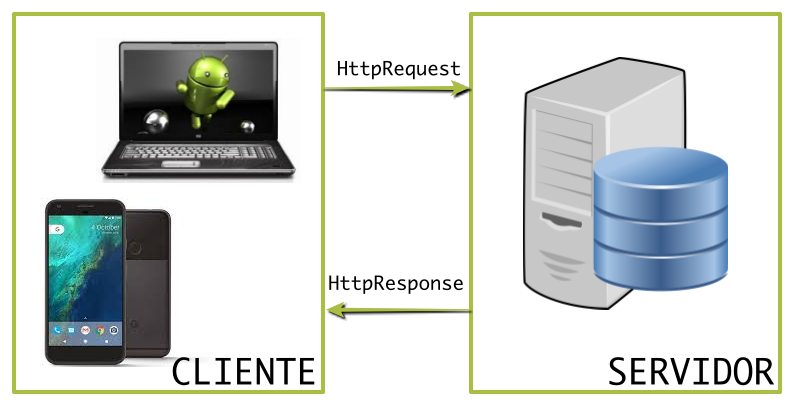
\includegraphics[width=7cm, keepaspectratio]{img/arquitectura}
  \caption{Arquitectura Cliente-Servidor}
  \label{fig:arquitectura}
\end{figure}

% DISEÑO E IMPLEMENTACIÓN DEL SERVIDOR %
\section{Diseño e implementación del servidor} 
\label{sec:arquitecturaServidor}
Como hemos visto, la arquitectura del Servidor consta de dos grandes bloques: la lógica de Django y el almacenamiento de SQLite.  

\subsection{Lógica servidor: Django}
La lógica del proyecto My App Inventor está organizada en los siguientes directorios:
\begin{itemize}
	\item Projecto Django - \textbf{analyzeMyApp}: dentro nos encontraremos con los ficheros de configuración. En \textit{settings.py} indicaremos los parámetros principales del programa (directorios, idioma, base de datos \ldots), mientras que en \textit{wsgi.py} especificaremos las reglas de comunicación entre un servidor web y nuestra aplicación cuando despleguemos en producción. 
	\item Aplicación - \textbf{myAnalyzer}: en este directorio guardaremos la lógica de la aplicación, es decir, qué hacer cuando recibimos una petición, cómo será nuestro modelo de datos, qué pasos seguir al analizar un fichero recibido\ldots. En las siguientes secciones veremos más en detalle este apartado.
	\item Ficheros estáticos - \textbf{static}: donde están las imágenes, estilos CSS y pequeños JavaScript para utilizar con Bootstrap.  
	\item Plantillas - \textbf{templates}: incluye todas las plantillas HTML que formarán parte de la interacción del usuario con la aplicación. 
	\item Proyectos guardados - \textbf{saved\_projects}: además de guardar la información más relevante en base de datos, guardaremos una copia de seguridad de cada proyecto subido por el usuario en disco, así en caso de posibles ampliaciones de la lógica de evaluación, se podrá actualizar el resultado de forma transparente al usuario sin necesidad de que vuelva a cargar su programa de nuevo. 
\end{itemize}  
\begin{figure}[H]
  \dirtree{%
	.1 /.
	.2 manage.py.
	.2 analyzeMyApp.
	.3 \_\_init\_\_.py.
	.3 settings.py.
	.3 urls.py.
	.3 wsgi.py.
	.2 myAnalyzer.
	.3 \_\_init\_\_.py.
	.3 admin.py.
	.3 scoreMyAppMessages.py.
	.3 admin.py.
	.3 forms.py.
	.3 models.py.
	.3 urls.py.
	.3 apps.py.
	.3 scoreMyApp.py.
	.3 parser.py.
	.3 views.py.
	.3 errors.py.
	.3 tests.py.
	.2 static.
	.2 templates.
	.2 saved\_projects.
	}
  \caption{Directorio de archivos My App Inventor}
  \label{fig:dirarchivos}
\end{figure}

En líneas generales, el flujo de la aplicación sigue los pasos de la Figura~\ref{fig:flujoapp} y se define dentro del directorio \textbf{myAnalyzer}. Cuando un usuario registrado realiza una petición a la aplicación, se diferencia entre guardar un nuevo proyecto o cargar uno preexistente. Tras este paso, se procede al anáĺisis del programa y como paso final, se devuelve una respuesta con la clasificación obtenida. Durante todo el proceso, si se recibe una petición de un usuario no registrado, se redirige al mismo a la página de inicio. 
\begin{figure}[H]
  \centering
  \begin{tikzpicture}[node distance = 3cm]
	    % Place nodes
	    \node [block] (init) {Petición de usuario};
	    \node [decision, below of= init] (newproject) {¿Nuevo projecto?};
	    \node (AuxNode01) [text width=4cm, below of=newproject] {};
	    \node [block, right of=AuxNode01, node distance=3cm] (save) {Guardar en bbdd};
	    \node [block, left of=AuxNode01, node distance=3cm] (load) {Leer de bbdd};
	    \node [block, below of=AuxNode01] (analyze) {Analizar proyecto};
	    \node [block, below of=analyze] (end) {Enviar resultados};
	    % Draw edges
	    \path [line] (init) -- (newproject);
	    \path [line] (newproject) -| node [near start, above] {si} (save);
	    \path [line] (newproject) -| node [near start, above]{no}(load);
	    \path [line] (load) -- (analyze);
	    \path [line] (save) -- (analyze);
	    \path [line] (analyze) -- (end);
  \end{tikzpicture}
  \caption{Flujo principal My App Inventor}
  \label{fig:flujoapp}
\end{figure}
En el momento en que la aplicación recibe una petición HTTP del usuario con una URL concreta, ésta se mapea en el fichero \textit{urls.py}. Éste a su vez redirige la información a un procedimiento concreto de \textit{wsgi.py} en función de la operación a realizar: iniciar o cerrar sesión, actualizar datos de perfil, cargar un nuevo programa, ver los anteriormente guardados \ldots No todas las URLs son accesibles al usuario mediante la petición GET; por ejemplo, sólo podremos acceder a la vista que analiza los proyectos del usuario,\textit{views.showUserAnalyzeProjectsPage}, mediante una petición de tipo POST insertada en un formulario de la aplicación para mantener la integridad de los datos recibidos y controlar su contenido. Lo mismo ocurre con la vista \textit{views.showDownloadPage} en la que se accede a la petición POST a través de un formulario.
\begin{lstlisting}
urlpatterns = [
               url(r'^login/', views.showLoginPage),
               url(r'^logout/', views.showLogoutPage),
               url(r'^createprofile/', views.showCreateProfilePage),
               url(r'^userprofile/', views.showUserProfilePage),
               url(r'^download/', views.showDownloadPage),
               url(r'^updateprofile/', views.showUpdateProfilePage),
               url(r'^userprojects/', views.showUserProjectsPage),
               url(r'^analyze/', views.showUserAnalyzeProjectsPage),
               url(r'^$', views.showLoginPage),
               ]
\end{lstlisting}

Veamos en más detalle los diferentes procedimientos implicados en el proceso global que forman parte de la aplicación.
\subsubsection{Comunicación}
Como hemos comentado anteriormente, si un usuario no inicia sesión en la aplicación, se le devolverá siempre a la página inicial. Entre todas las librerías (o \textit{views}) que incorpora Django, utilizaremos el Sistema de Autenticación \footnote{\url{https://docs.djangoproject.com/en/1.11/topics/auth/default/}} para complementar las vistas que nos ayudarán a realizar las operaciones más comunes como iniciar o cerrar sesión (\textit{views.showLoginPage, views.showLogoutPage}), mantener la misma entre peticiones al servidor o comprobar si un usuario está conectado. 

Todas las peticiones se realizarán a través de los objetos HttpResponse \footnote{\url{https://docs.djangoproject.com/en/1.11/ref/request-response/}} de Django que manejan solicitudes GET y POST según corresponda. Por ejemplo, en la vista de inicio de sesión, se diferencia entre la solicitud de \textit{login} (GET), donde respondemos al usuario con un formulario en el que introducir sus datos de registro, y la recepción de los mismos en el método POST para autenticarle. 

Tras el inicio de sesión, el usuario será redirigido a la página principal donde podrá evaluar su código en función de si ya está subido a la aplicación o no, como vimos en la Figura~\ref{fig:flujoapp}. 

\begin{figure}[H]
  \centering
  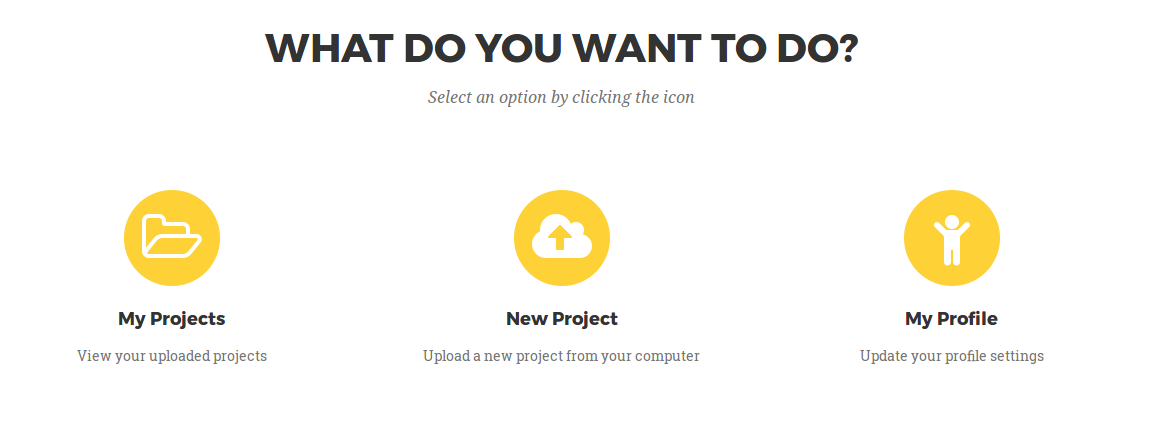
\includegraphics[width=\linewidth, keepaspectratio]{img/usercontent}
  \caption{Opciones disponibles}
  \label{fig:usercontent}
\end{figure}

Primero veamos el caso donde un programador quiere analizar su código por primera vez. La función \textit{views.showDownloadPage} devuelve en la primera petición (GET) un formulario en el que el usuario podrá buscar en su disco el fichero comprimido \textit{.aia} que previamente se ha descargado de su cuenta en App Inventor. Tras pulsar el botón Enviar, el navegador enviará una petición POST con el fichero al Servidor, donde se comprobará que no existe previamente para este usuario y descomprimirá, para posteriormente almacenar la información más relevante en base de datos. 

La estructura en la que App Inventor guarda la información sigue el esquema descrito en la figura~\ref{fig:dirappinventor}. En la carpeta \textit{assets} se almacenan los ficheros estáticos de la aplicación, como las imágenes y sonidos. En \textit{project.properties} se especifica la configuración del proyecto: versión del código, primera pantalla, tamaño\ldots. Y finalmente en el último nivel del directorio \textit{src} se encuentran la información relativa a los bloques utilizados (*.scm) y las lógicas que los relacionan (*.bky) por pantallas. Los datos más importantes para My App Inventor se encuentran en este último nivel y por ello serán los que guardemos en base de datos para su posterior análisis. 

\begin{figure}[H]
  \dirtree{%
	.1 /.
	.2 assets.
	.2 src.
	.3 appinventor.
	.4 settings.py.
	.5 ai\_loginappinventor.
	.6 nombrePrograma.
	.7 fichero.bky.
	.7 fichero.scm.
	.7 \ldots.
	.2 youngandroidproject.
	.3 project.properties.
	}
  \caption{Directorio App Inventor}
  \label{fig:dirappinventor}
\end{figure}

Si en un primer caso partíamos de un nuevo fichero de código, nuestra aplicación también permite al usuario guardar los proyectos guardados para poder volver a analizarlos en el futuro. Al llamar a la función \textit{views.showUserProjectsPage} el Servidor listará todos los programas almacenados para el usuario y éste podrá volver a obtener su clasificación. 

Tanto si partimos de un código nuevo como de uno ya existente, la última operación que hace My App Inventor es analizar el código. ¿Y por qué analizar algo que ya está puntuado? Pensando en futuras mejoras e implementaciones del algoritmo de análisis, de esta forma hacemos posible que el usuario siempre tenga su disposición la última versión del mismo con la clasificación más actualizada. Así no es necesario preprocesar todos los programas en base de datos en caso de actualización ya que ésta se realiza bajo demanda.

\subsubsection{Análisis de código}
El análisis de los programas del usuario se realiza a tres niveles: componentes, programación y usabilidad, cada uno con sus correspondientes subniveles. Como habíamos comentado en la sección anterior, en base de datos tendremos la información principal de las pantallas que forman cada proyecto. Para cada pantalla tenemos:

\begin{itemize}
  \item Fichero \textbf{.scm}: contiene los bloques añadidos al proyecto y sus propiedades en formato JSON (JavaScript Object Notation)\footnote{\url{http://www.json.org/}}, un formato de representación de objetos con una estructura sencilla basada en relaciones nombre-valor. En función del bloque utilizado tendremos unas propiedades u otras: posición (\textit{AlignHorizontal}), fondo (\textit{BackgroundColor}), tamaño (\textit{Width}) \ldots 
	\begin{figure}[H]
	  \centering
	  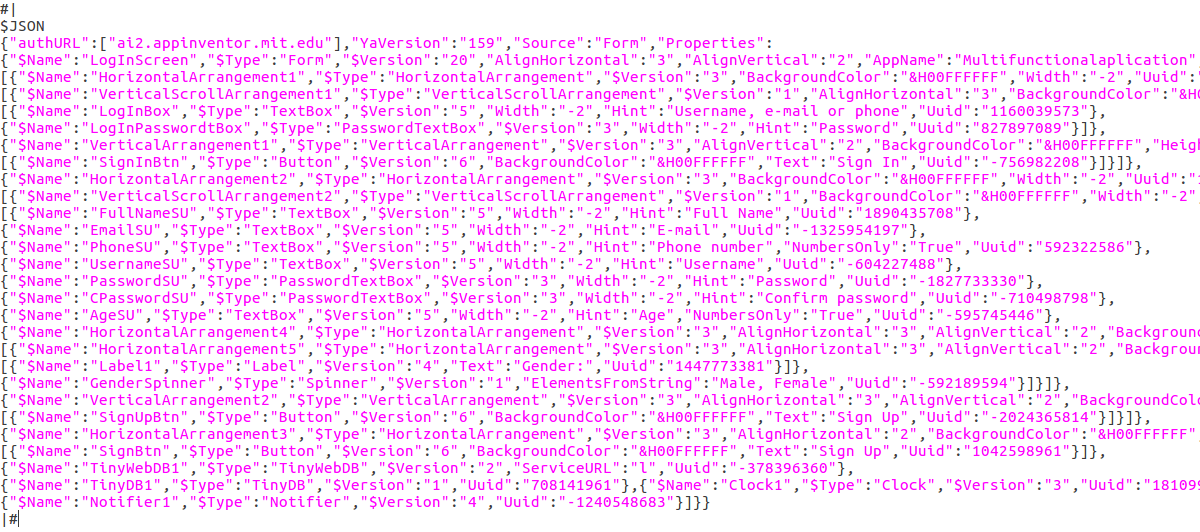
\includegraphics[width=\linewidth, keepaspectratio]{img/scmCode}
	  \caption{Ejemplo fichero .scm}
	  \label{fig:scmfile}
	\end{figure}
  \item Fichero \textbf{.bky}: en él se almacena en formato XML (Extensible Markup Language)\footnote{\url{https://www.w3.org/XML/}} todas las relaciones entre bloques activos y su funcionamiento. Será por tanto el principal fichero del que extraeremos la información estructural y funcional a analizar.
	\begin{figure}[H]
	  \centering
	  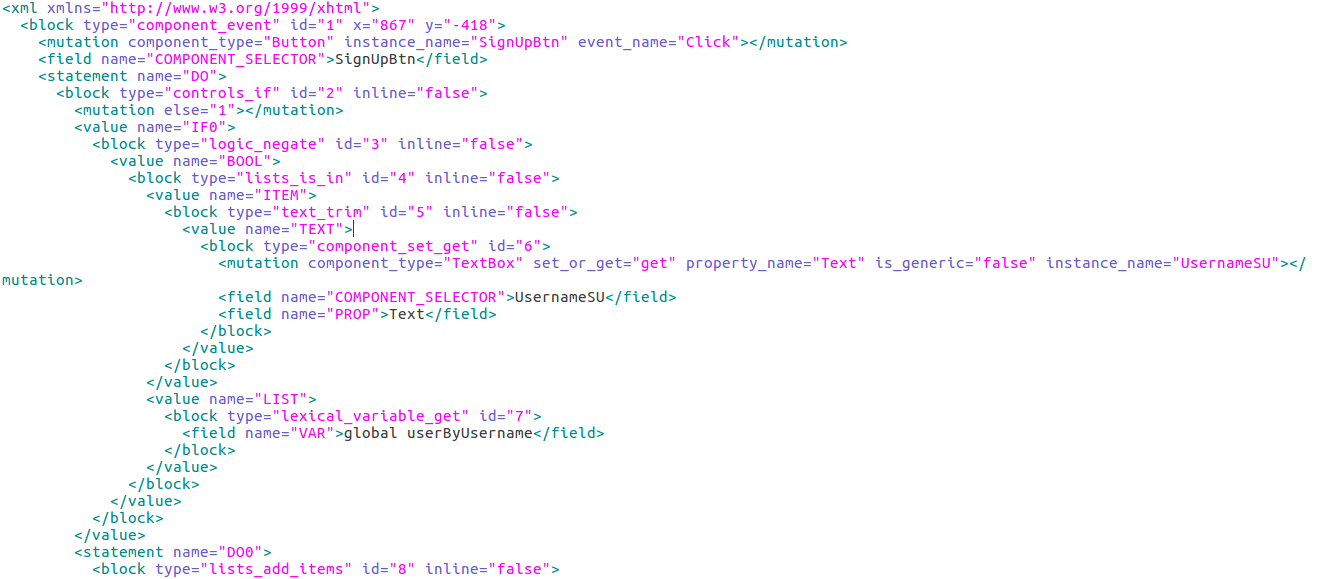
\includegraphics[width=\linewidth, keepaspectratio]{img/bkyCode}
	  \caption{Ejemplo fichero .bky}
	  \label{fig:bkyfile}
	\end{figure}
\end{itemize}

La función \textit{views.showUserAnalyzeProjectsPage} será la encargada de recibir la identificación del proyecto a analizar y responder al usuario con su evaluación. Tras consultar el contenido de las pantallas en base de datos, llamará a la función \textit{scoreMyApp.getScore} que analizará cada nivel individualmente. En este proceso, las funciones llamadas se han organizado en diferentes clases según su propósito:
\begin{itemize}
  \item \textbf{scoreMyApp}: contiene todas las funciones relativas a analizar el XML y obtener las estadísticas. Su función principal es \textit{scoreMyApp.getScore} y en esta sección nos centraremos en su análisis. 
  \item \textbf{scoreMyAppMessages}: procesa las clasificaciones y genera mensajes personalizados para el usuario.
\end{itemize}

Dentro de \textit{scoreMyApp.getScore} analizaremos cada nivel pantalla por pantalla, comparando los resultados en cada iteración de forma que la estructura final contenga toda la información del programa. 
\begin{lstlisting}
if componentLevels['Score'] > generalScore['ComponentLevels']['Score']:
# Update
generalScore['ComponentLevels']['Score'] = componentLevels['Score']

G1 = generalScore['ComponentLevels']['L1_components']
S1 = componentLevels['L1_components']
generalScore['ComponentLevels']['L1_components'] = returnUnion(G1,S1,0)
\end{lstlisting}
La clasificación se almacenará en un diccionario en el que guardaremos las estadísticas de cada nivel. Para obtener las puntuaciones individuales se obtiene una media con los niveles de las clasificaciones, mientras que la puntuación final es una media ponderada de los tres niveles a analizar. Los componentes utilizados y las habilidades de programación tienen un peso del 45\% cada uno en la media mientras que la usabilidad de la aplicación se lleva el 10\% restante al considerarse una característica a evaluar pero que no debe tener la misma importancia en la nota final pues es un concepto más de diseño que de habilidad en la programación.  
\begin{figure}[H]
	\begin{center}
	    \begin{tabular}{| l | l | l | }
	    \hline
	    \textbf{Nivel} & \textbf{Subniveles} & \textbf{Ponderación} \\ \hline
	    ComponentLevels & Score,L1\_components,L2\_components,L3\_components & 45\% \\ \hline
	    ProgrammingLevels & Score,Flow,Data,Variable,Generalization & 45\% \\ \hline
	    ScreensLevels & Score,Screens & 10\% \\ \hline
            \end{tabular}
	\end{center}
	\caption{Estructura de la clasificación}
	\label{fig:scoreStructure}
\end{figure}

Para la evaluación de los \textbf{componentes} se han clasificado en tres niveles todos los bloques disponibles en App Inventor en función de su nivel de complejidad, independientemente de su naturaleza. Por ejemplo, en el nivel Bajo nos encontramos con bloques tipo cuadro de texto y relojes, mientras que en el nivel Alto tenemos componentes de Lego Mindstorms o bases de datos experimentales como FirebaseDB. 

\begin{figure}[H]
	\begin{center}
	    \begin{tabular}{| l | p{0.85\linewidth} | }
	    \hline
	    \textbf{Subnivel} & \textbf{Bloques} \\ \hline
		Bajo & \textbf{InterfazUsuario} [Button CheckBox DatePicker Image Label ListPicker ListView Notifier Slider Spinner TextBox TimePicker] \textbf{Diseño} [HorizontalArrangement HorizontalScrollArrangement TableArrangement VerticalArrangement VerticalScrollArrangement] \textbf{Media} [ImagePicker] \textbf{Dibujo} [Ball Canvas ImageSprite] \textbf{Sensores} [Clock] \\ \hline
		Medio & \textbf{InterfazUsuario} [PasswordTextBox WebViewer] \textbf{Media} [Camcorder Camera Player Sound SoundRecorder SpeechRecognizer TextToSpeech VideoPlayer YandexTranslate] \textbf{Sensores} [AccelerometerSensor BarcodeScanner OrientationSensor Pedometer] \textbf{Social} [ContactPicker EmailPicker PhoneCall PhoneNumberPicker Sharing Texting Twitter] \textbf{Almacenamiento} [File TinyDB] \textbf{Conectividad} [ActivityStarter BluetoothClient]\\ \hline
		Alto & \textbf{Sensores} [GyroscopeSensor LocationSensor NearField ProximitySensor] \textbf{Almacenamiento} [FusionTablesControl TinyWebDB] \textbf{Conectividad} [BluethoothServer Web] \textbf{Lego} [NctDrive NctColorSensor NxtLightSensor NxtSoundSensor NxtTouchSensor NxtUltrasonicSensor NxtDirectCommands Ev3Motors Ev3ColorSensor Ev3GyroSensor Ev3TouchSensor Ev3UltrasonicSensor Ev3Sound Ev3UI Ev3Commands] \textbf{Experimental} [FirebaseDB]\\ \hline
            \end{tabular}
	\end{center}
	\caption{Componentes}
	\label{fig:componentsScore}
\end{figure}

Una vez definidos los tres niveles, con la función \textit{scoreMyApp.componentLevels\_Score} buscaremos todas las ocurrencias de cada tipo de bloque dentro de la pantalla, guardando los resultados en tres diccionarios:
\begin{lstlisting}
L1_found = {'UserInterface': UserInterface_L1_found,
                'Layout': Layout_L1_found,
                'Media': Media_L1_found,
                'Drawing': Drawing_L1_found,
                'Sensors': Sensors_L1_found}
    
L2_found = {'UserInterface': UserInterface_L2_found,
        'Media': Media_L2_found,
        'Sensors': Sensors_L2_found,
        'Social': Social_L2_found,
        'Storage': Storage_L2_found,
        'Connectivity':Connectivity_L2_found}
    
L3_found = {'Sensors': Sensors_L3_found,
        'Storage': Storage_L3_found,
        'Connectivity':Connectivity_L3_found,
        'Lego':Lego_L3_found,
        'Experimental':Experimental_L3_found}
\end{lstlisting}
Tras contabilizar el número de componentes total en cada subnivel, se asignará la puntuación de este módulo en función de la nota máxima alcanzada y guardaremos tanto la puntuación como el análisis para poder utilizarlos más adelante.   
\begin{lstlisting}
if c3 > 0 : # High score for complex components
score = 3
elif c2 > 0: # Medium score for complicated components
score = 2
else: # Low score for simple components
score = 1

results = {'Score':score,
       'L1_components':L1_found,
       'L2_components': L2_found,
       'L3_components': L3_found}
\end{lstlisting}

En la \textbf{programación} se revisarán competencias del usuario en distintas áreas de caracter abstracto como el control de flujo o el uso de funciones. Se han intentado agrupar a alto nivel las posibles etiquetas para poder organizarlas por funcionalidad y dentro de la misma, en los mínimos grupos, de manera que para cada subnivel tendremos siempre dos grupos globales que nos ayudarán a determinar la puntuación. 
\begin{figure}[H]
	\begin{center}
	    \begin{tabular}{| l | p{0.80\linewidth} | }
	    \hline
	    \textbf{Subnivel} & \textbf{Identificadores} \\ \hline
		Flow & component\_event controls\_ \\ \hline
		Data & lists component\_set\_get \\ \hline
		Variable & global\_declaration lexical\_variable\_get lexical\_variable\_set math\_ text\_ local\_declaration\_statement local\_declaration\_expression \\ \hline
		Generalization & procedures\_ is\_generic \\ \hline
            \end{tabular}
	\end{center}
	\caption{Programación}
	\label{fig:programmingScore}
\end{figure}
\begin{itemize}
  \item \textbf{Control de flujo} \textit{scoreMyApp.flow\_control}: identifica las expresiones lógicas para ejecutar ciclos, estructuras condicionales o eventos que dependen del comportamiento de otro componente o variable.
	\begin{itemize}
		\item Nivel alto: se incluyen expresiones lógicas y eventos dependientes. 
		\item Nivel medio: se incluyen expresiones lógicas o eventos dependientes.
		\item Nivel bajo: no incluye ningún control de flujo. 
	\end{itemize}
  \item \textbf{Gestión de datos} \textit{scoreMyApp.data\_control}: detecta el uso de listas para organización datos y asignación o modificación de valores a variables y componentes.
	\begin{itemize}
		\item Nivel alto: se incluyen listas y modificadores de variables. 
		\item Nivel medio: se incluyen listas o modificadores de variables.
		\item Nivel bajo: no se utilizan etiquetas de gestión de datos. 
	\end{itemize}
  \item \textbf{Representación de variables} \textit{scoreMyApp.variable\_control}: se tendrá en cuenta si el usuario utiliza declaraciones de variables tanto globales como locales y, en función del tipo de programa, expresiones matemáticas (sumas, potencias, operaciones de trigonometría\ldots) o expresiones relacionadas con textos (unión, convertir a mayúsculas, contiene\ldots).
	\begin{itemize}
		\item Nivel alto: se incluyen declaración de variables y funcionalidades de matemáticas o texto. 
		\item Nivel medio: se incluyen declaración de variables o funcionalidades de matemáticas o texto.
		\item Nivel bajo: no se utilizan métodos referenciados a variables. 
	\end{itemize}
  \item \textbf{Generalización} \textit{scoreMyApp.generalization\_control}: la optimización de código a través de funciones y la generalización de procesos para un mismo tipo de variable son características que todo buen programa debe tener ya que facilitan su lectura y permiten la reutilización procedimientos.   
	\begin{itemize}
		\item Nivel alto: se incluyen procedimientos y eventos genéricos para un mismo tipo de componente. 
		\item Nivel medio: se incluyen procedimientos (en esta ocasión se ha considerado que el uso de procedimientos es una funcionalidad básica e imprescindible)
		\item Nivel bajo: no se utiliza ningún tipo de mecanismo de generalización. 
	\end{itemize}
\end{itemize}
Al igual que en el nivel anterior, se guardarán todas las estadísticas e identificadores obtenidos en un diccionario además de la nota media de todas las subcategorías:
\begin{lstlisting}
results = {'Score':score,
       'Flow': flowCtrl,
       'Data': dataCtrl,
       'Variable': variableCtrl,
       'Generalization': generalizationCtrl}
\end{lstlisting}

Por último analizaremos la \textbf{usabilidad} extrapolándola al número de pantallas que forman la aplicación. Una de la características de las aplicaciones actuales es su simplicidad para el usuario. Incluir gran cantidad de pantallería y opciones reduce su usabilidad al convertirla en poco intuitiva. Si queremos mejorar la experiencia de usuario conviene que nuestro programa tenga un número suficientemente bajo de pantallas para que resulte fácil de utilizar pero no sea excesivamente sencillo para que no pierda funcionalidad. Tras estudiar las aplicaciones existentes en el mercado, en este apartado se han definido los siguientes niveles dentro de la función \textit{scoreMyApp.nScreens\_control}:
\begin{itemize}
	\item Nivel alto: entre 3 y 10 pantallas distintas. Ejemplos: Twitter, Facebook, Instagram\ldots
	\item Nivel medio: entre 1 y 3 pantallas. Ejemplos: Notas, Reloj, Calculadora
	\item Nivel bajo: una única pantalla.  
\end{itemize}

Tras el análisis de los componentes, técnicas de programación y usabilidad para todas las pantallas que componen el programa a analizar, obtendremos el siguiente esquema de resultados recopilando la máxima información posible:
\begin{figure}[H]
  \dirtree{%
	.1 GeneralScore.
	.2 ComponentLevels.
	.3 Score.
	.3 L1\_components.
	.3 L2\_components.
	.3 L3\_components.
	.2 ProgrammingLevels.
	.3 Score.
	.3 Flow.
	.4 Component\_Events.
	.4 Control.
	.3 Data.
	.4 Lists.
	.4 ComponentSet.
	.3 Variable.
	.4 Variable.
	.4 Math.
	.4 Text.
	.3 Generalization.
	.4 Procs.
	.4 Generic.
	.2 ScreensLevels.	
	.3 Score.
	.3 Screens.
	}
  \caption{Resultados del análisis}
  \label{fig:scoreAppInventor}
\end{figure}
\subsubsection{Envío de resultados}
Volviendo a la vista encargada de obtener los resultados finales, \textit{views.showUserAnalyzeProjectsPage}, tras el análisis de los ficheros que componen el programa, llamaremos a las funciones de la clase \textit{scoreMyAppMessages}. En ella procesaremos toda la información y la mostraremos al usuario de forma intuitiva y simplificada a través de imágenes y mensajes de texto cortos. 
 
Gracias a la función \textit{scoreMyAppMessages.getScoreMsgs} obtendremos todos los datos necesarios que queremos mostrar al usuario a partir de los resultados vistos en el apartado anterior:
\begin{itemize}
	\item Nivel global - \textit{general\_score\_msg}: a partir de la puntuación general tendremos un mensaje que resumirá el nivel promedio de la aplicación. 
		\begin{lstlisting}
# General Score message
if score['Score'] == 3:
	general_score_msg = 'Great job! Your app has a HIGH score! Check out the different skills to improve it even more'
elif score['Score'] == 2:
	general_score_msg = 'Great job! Your app has a MEDIUM score! Check out the different skills to reach the next level'
else:
	general_score_msg = 'Ups! Your app has a LOW score. Check out the different skills to improve it'
		\end{lstlisting}
	\item Nivel por categoría - \textit{comp\_score\_msg, progr\_score\_msg, sched\_score\_msg}: componentes, programación y usabilidad mostrarán un mensaje personalizado en función de la puntuación media de sus subniveles. 
	\item Desglose de resultados por categoría - \textit{comp\_score\_info, progr\_score\_info, sched\_score\_info}: cada apartado incluirá la información más importante del mismo además de un consejo para mejorar el nivel actual. Dicho mensaje se mostrará siempre, pues aunque el usuario haya obtenido la máxima puntuación trataremos de motivarle para que incluya más complejidad a su programa o mayor diversidad de componentes. 
	\begin{itemize}
		\item Componentes: listará los bloques utilizados para conseguir este nivel.  
		\begin{figure}[H]
			  \centering
			  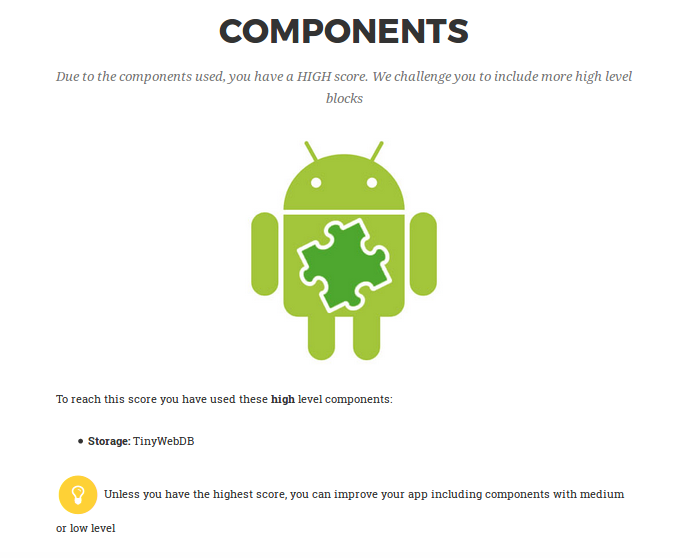
\includegraphics[width=0.50\linewidth, keepaspectratio]{img/componentsScore}
			  \caption{Resultados de la categoría Componentes}
			  \label{fig:compResults}
		\end{figure} 
		\item Programación: resumirá por categorías todos los identificadores añadidos al código junto con el número de veces que se utilizan de forma que el usuario pueda tener una visión global la estructura de su programa.      
		\begin{figure}[H]
			  \centering
			  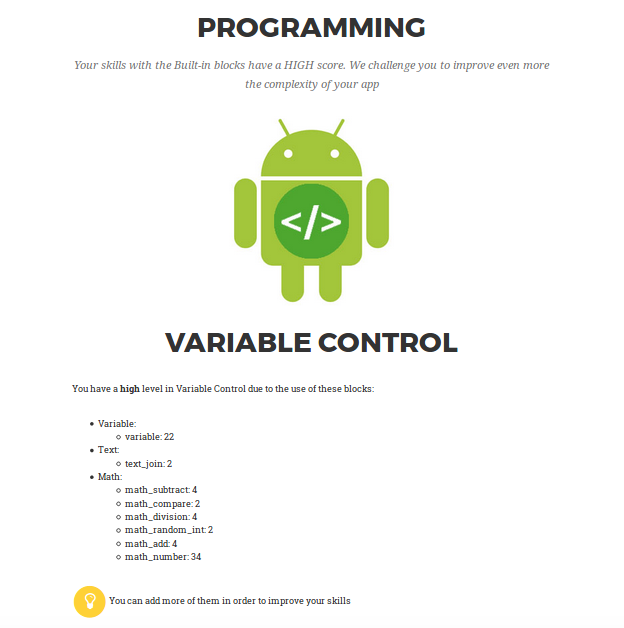
\includegraphics[width=0.60\linewidth, keepaspectratio]{img/programmingScore}
			  \caption{Resultados de la categoría Programación}
			  \label{fig:progrResults}
		\end{figure} 
		\item Usabilidad: muestra el número de pantallas que forman el programa.       
		\begin{figure}[H]
			  \centering
			  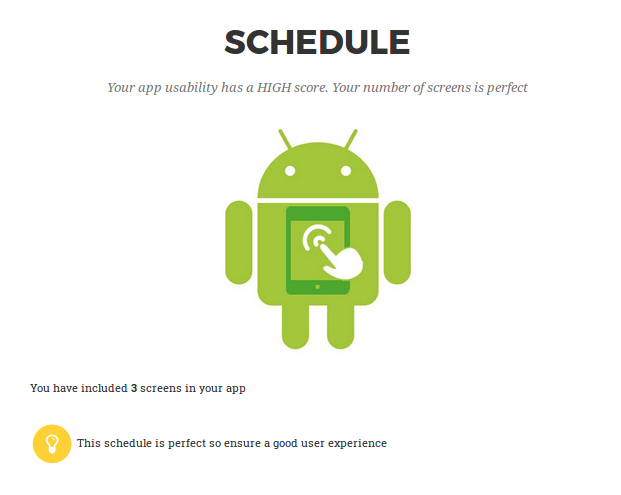
\includegraphics[width=0.50\linewidth, keepaspectratio]{img/schedScore}
			  \caption{Resultados de la categoría Usabilidad}
			  \label{fig:schedResults}
		\end{figure} 
	\end{itemize}
\end{itemize}

Una vez obtenidos todos los resultados, el siguiente pasó será enviarlos al navegador del usuario a través de la página \textit{analyzeAppCode.html}.En ésta se unen la mayoría de las tecnologías vistas en el capítulo Estado del Arte:
\begin{itemize}
	\item HTML: como estándar para definir la estructura básica del archivo, legible e interpretable por el navegador. Identificado en la siguiente etiqueta dentro del propio fichero:	
		\begin{lstlisting}
<!DOCTYPE html>
		\end{lstlisting}
	\item CSS: antes de enviar el archivo HMTL, parsearemos tanto los resultados del análisis como el estilo para integrarlos con el resto de valores de la página. Todos los formatos estarán definidos en diferentes ficheros .css almacenados estáticamente en el Servidor.  
		\begin{lstlisting}


...

<link href="" rel="stylesheet">
		\end{lstlisting}
	\item JavaScript: gracias a este lenguaje de programación podemos implementar funciones dentro del HTML para que nuestra página sea más dinámica. Se utiliza por ejemplo, a la hora de ocultar o mostrar el menú:
	\begin{lstlisting}
... 

// Highlight the top nav as scrolling occurs
$('body').scrollspy({
	target: '.navbar-fixed-top',
	offset: 51 });

// Closes the Responsive Menu on Menu Item Click
$('.navbar-collapse ul li a').click(function(){ 
    $('.navbar-toggle:visible').click(); });
	\end{lstlisting}
	\item Bootstrap: \textit{framework} que aúna el resto de tencnologías (HTML, CSS, JavaScript) y nos permite que la página se adapte a dispositivos móviles como se muestra en la figura~\ref{fig:dirappinventor}.
		\begin{lstlisting}
    <!-- Bootstrap Core CSS -->
    <link href="" rel="stylesheet">
		\end{lstlisting}
		\begin{figure}[H]
			  \centering
			  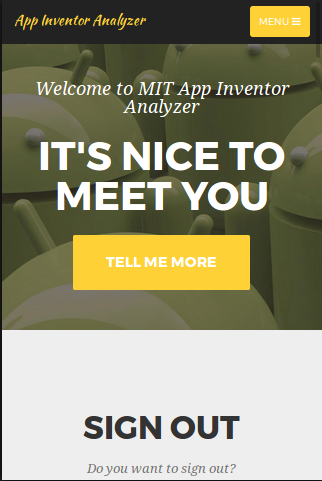
\includegraphics[width=0.30\linewidth, keepaspectratio]{img/mobileVersion}
			  \caption{Versión móvil con Bootstrap}
			  \label{fig:mobileVersion}
		\end{figure} 
		\begin{figure}[H]
			  \centering
			  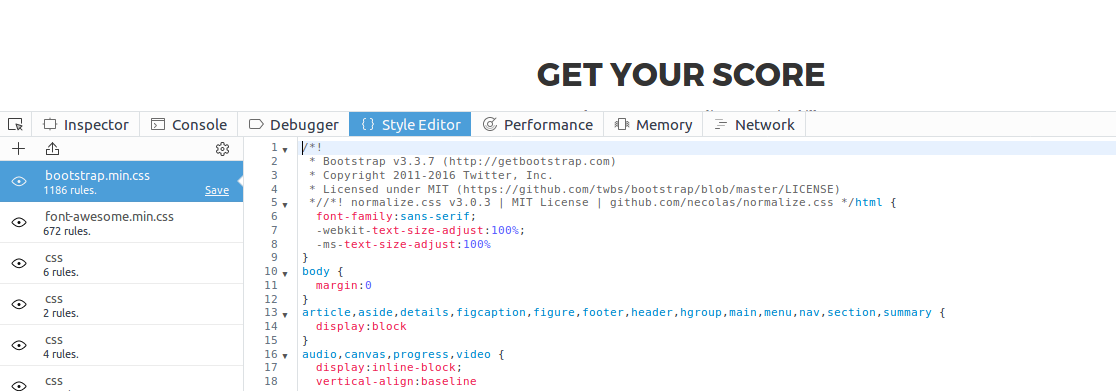
\includegraphics[width=\linewidth, keepaspectratio]{img/bootstrapDebug}
			  \caption{Petición de Bootstrap desde el navegador}
			  \label{fig:mobileVersion}
		\end{figure} 

\end{itemize}                                   

\subsection{Modelo de datos}
En la organización y uso de la información se han utilizado dos modelos en función de las características de los datos a guardar: 
\begin{itemize}
	\item Contenido no persistente: variables locales creadas durante la ejecución de los procesos en el servidor. 
	\item Contenido persistente: base de datos SQLite\footnote{\url{https://www.sqlite.org}} y almacenamiento en memoria.
\end{itemize}                                   

Como vimos en la sección anterior, los datos dinámicos donde se almacenan los resultados tras el análisis de código se guardan en una variable de tipo diccionario, donde se organizarán en pares clave-valor. En ella tendremos acceso tanto a las puntuaciones como a las prácticas de programación que las originan, ambas respresentadas en la figura~\ref{fig:scoreAppInventor}.

Por otro lado tendremos el almacenamiento en memoria estática de los programas subidos por cada usuario. Para ello se ha creado un sistema de directorios donde ir descargando el código y así poder tener acceso a él en el futuro en caso de actualizaciones del sistema de análisis. 

Los datos relativos a la información de usuario o los proyectos guardados por el mismo se guardarán en una base de datos, definida dentro de la aplicación en las clases de \textit{models.py}. Para todo lo relativo a la creación y autenticación de usuarios, Django dispone de objetos predefinidos \footnote{\url{https://docs.djangoproject.com/en/1.11/topics/auth}} que se han reutilizado añadiendo nuevas características. Para el caso del objeto User, que por defecto incluye como atributos primarios \textit{username, password, email, first\_name} y \textit{last\_name}, se ha usado de modelo base para la clase \textit{UserProfile} extendiéndolo de forma que también incluya el campo \textit{appinventorLogin}, necesario en la extracción de los ficheros comprimidos subidos por el usuario.
\begin{lstlisting}
class UserProfile(models.Model):
    user = models.OneToOneField(User)

    # The additional attributes we wish to include.
    appinventorLogin = models.CharField(max_length =254 )

    # Override the __unicode__() method to return out something meaningful!
    def __unicode__(self):
        return self.user.username    
\end{lstlisting}
Para almacenar los usuarios existentes en la aplicación, sus proyectos y el contenido de los mismos se han creado las siguientes clases: 
\begin{lstlisting}
class Users(models.Model):
    userID = models.IntegerField(primary_key=True) # user_id
    projects = models.ManyToManyField('Projects') # The user can load and analyze multiple projects

class Projects(models.Model):
    projectName = models.TextField(primary_key=True) # user.id_filename.name
    screens = models.ManyToManyField('Screens') # The project can include multiple screens
    projectProperties = models.TextField() # Project properties
    
class Screens(models.Model):
    scrID = models.TextField(primary_key=True) # user.id_filename.name_Screen number
    bky = models.TextField() # Blockly info
    scm = models.TextField() # Screen Description
\end{lstlisting} 
De esta forma un usuario puede tener varios proyectos que a su vez estarán compuestos por una o varias pantallas asociadas:
\begin{figure}[H]
  	\centering
	\begin{tikzpicture}[node distance = 3cm]
	    % Place nodes
	    \node [block] (init) {Users};
	    \node [block, below of=init] (project) {Projects};
	    \node [block, below of=project] (screens) {Screens};
	    % Draw edges
	    \path [line] (init) -- (project);
	    \path [line] (project) -- (screens);
	\end{tikzpicture}
	\caption{Modelo de datos}
	\label{fig:databasemodel}
\end{figure}


% MANUAL DE USUARIO %
\section{Manual de Usuario} 
\label{sec:manualUsuario}

%%%%%%%%%%%%%%%%%%%%%%%%%%%%%%%%%%%%%%%%%%%%%%%%%%%%%%%%%%%%%%%%%%%%%%%%%%%%%%%%
%%%%%%%%%%%%%%%%%%%%%%%%%%%%%%%%%%%%%%%%%%%%%%%%%%%%%%%%%%%%%%%%%%%%%%%%%%%%%%%%
% RESULTADOS %
%%%%%%%%%%%%%%%%%%%%%%%%%%%%%%%%%%%%%%%%%%%%%%%%%%%%%%%%%%%%%%%%%%%%%%%%%%%%%%%%

\cleardoublepage
\chapter{Resultados}




%%%%%%%%%%%%%%%%%%%%%%%%%%%%%%%%%%%%%%%%%%%%%%%%%%%%%%%%%%%%%%%%%%%%%%%%%%%%%%%%
%%%%%%%%%%%%%%%%%%%%%%%%%%%%%%%%%%%%%%%%%%%%%%%%%%%%%%%%%%%%%%%%%%%%%%%%%%%%%%%%
% CONCLUSIONES %
%%%%%%%%%%%%%%%%%%%%%%%%%%%%%%%%%%%%%%%%%%%%%%%%%%%%%%%%%%%%%%%%%%%%%%%%%%%%%%%%

\cleardoublepage
\chapter{Conclusiones}
\label{chap:conclusiones}


\section{Consecución de objetivos}
\label{sec:consecucion-objetivos}

Esta sección es la sección espejo de las dos primeras del capítulo de objetivos,
donde se planteaba el objetivo general y se elaboraban los específicos.

Es aquí donde hay que debatir qué se ha conseguido y qué no. Cuando algo no
se ha conseguido, se ha de justificar, en términos de qué problemas se han
encontrado y qué medidas se han tomado para mitigar esos problemas.


\section{Aplicación de lo aprendido}
\label{sec:aplicacion}

Aquí viene lo que has aprendido durante el Grado/Máster y que has aplicado
en el TFG/TFM. Una buena idea es poner las asignaturas más relacionadas y
comentar en un párrafo los conocimientos y habilidades puestos en práctica.

\begin{enumerate}
  \item a
  \item b
\end{enumerate}


\section{Lecciones aprendidas}
\label{sec:lecciones_aprendidas}

Aquí viene lo que has aprendido en el Trabajo Fin de Grado/Máster.

\begin{enumerate}
  \item a
  \item b
\end{enumerate}


\section{Trabajos futuros}
\label{sec:trabajos_futuros}

Ningún software se termina, así que aquí vienen ideas y funcionalidades
que estaría bien tener implementadas en el futuro.

Es un apartado que sirve para dar ideas de cara a futuros TFGs/TFMs.


\section{Valoración personal}
\label{sec:valoracion}

Finalmente (y de manera opcional), hay gente que se anima a dar su punto de
vista sobre el proyecto, lo que ha aprendido, lo que le gustaría haber aprendido,
las tecnologías utilizadas y demás.



%%%%%%%%%%%%%%%%%%%%%%%%%%%%%%%%%%%%%%%%%%%%%%%%%%%%%%%%%%%%%%%%%%%%%%%%%%%%%%%%
%%%%%%%%%%%%%%%%%%%%%%%%%%%%%%%%%%%%%%%%%%%%%%%%%%%%%%%%%%%%%%%%%%%%%%%%%%%%%%%%
% APÉNDICE(S) %
%%%%%%%%%%%%%%%%%%%%%%%%%%%%%%%%%%%%%%%%%%%%%%%%%%%%%%%%%%%%%%%%%%%%%%%%%%%%%%%%

\cleardoublepage
\appendix
\chapter{Manual de usuario}
\label{app:manual}


%%%%%%%%%%%%%%%%%%%%%%%%%%%%%%%%%%%%%%%%%%%%%%%%%%%%%%%%%%%%%%%%%%%%%%%%%%%%%%%%
%%%%%%%%%%%%%%%%%%%%%%%%%%%%%%%%%%%%%%%%%%%%%%%%%%%%%%%%%%%%%%%%%%%%%%%%%%%%%%%%
% BIBLIOGRAFIA %
%%%%%%%%%%%%%%%%%%%%%%%%%%%%%%%%%%%%%%%%%%%%%%%%%%%%%%%%%%%%%%%%%%%%%%%%%%%%%%%%

\cleardoublepage

% Las siguientes dos instrucciones es todo lo que necesitas
% para incluir las citas en la memoria
\bibliographystyle{abbrv}
\bibliography{memoria}  % memoria.bib es el nombre del fichero que contiene
% las referencias bibliográficas. Abre ese fichero y mira el formato que tiene,
% que se conoce como BibTeX. Hay muchos sitios que exportan referencias en
% formato BibTeX. Prueba a buscar en http://scholar.google.com por referencias
% y verás que lo puedes hacer de manera sencilla.
% Más información: 
% http://texblog.org/2014/04/22/using-google-scholar-to-download-bibtex-citations/

\end{document}L
